\begin{center}
	\textbf{{\Huge ĐỀ ÔN TẬP GIỮA KÌ I LỚP 11}}
\end{center}
\subsubsection*{Phần I. Thí sinh trả lời từ câu 1 đến câu 12, mỗi câu hỏi chọn một phương án.}
\setcounter{bt}{0}\setcounter{bt}{0}\setlist[enumerate,1]{label=\quad\bfseries\Alph*.}
\begin{baitap}
	%\textbf{Câu 1:}
	Dãy số nào sau đây là một cấp số cộng?
	\begin{multicols}{2}
		\begin{enumerate}
			\item $(u_n): \begin{cases} u_1 = 1 \\ u_{n+1} = u_n + 2, \forall n \ge 1 \end{cases}$.
			\item $(u_n): \begin{cases} u_1 = 3 \\ u_{n+1} = 2u_n + 1, \forall n \ge 1 \end{cases}$.
			\item $(u_n): 1; 3; 6; 10; 15; \ldots$.
			\item $(u_n): -1; 1; -1; 1; -1; \ldots$.
		\end{enumerate}
	\end{multicols}
	\begin{traloi}
		\dapan{A}
		Dãy số $(u_n)$ xác định bởi $u_1 = 1$ và $u_{n+1} = u_n + 2$ với mọi $n \ge 1$ có $u_{n+1} - u_n = 2$ không đổi, nên là một cấp số cộng với công sai $d = 2$.
	\end{traloi}
\end{baitap}

\begin{baitap}
	%\textbf{Câu 2:}
	Cho cấp số cộng $(u_n)$ có $u_1 = \frac{1}{3}$, $u_8 = 26$. Tìm công sai $d$.
	\begin{multicols}{4}
		\begin{enumerate}
			\item $d = \frac{11}{3}$.
			\item $d = \frac{10}{3}$.
			\item $d = \frac{3}{10}$.
			\item $d = \frac{3}{11}$.
		\end{enumerate}
	\end{multicols}
	\begin{traloi}
		\dapan{A}
		Ta có $u_8 = u_1 + 7d \Rightarrow 26 = \frac{1}{3} + 7d \Rightarrow 7d = \frac{77}{3} \Rightarrow d = \frac{11}{3}$.
	\end{traloi}
\end{baitap}

\begin{baitap}
	%\textbf{Câu 3:}
	Cho $\tan \alpha = 2$. Tính $\tan \left(\alpha - \frac{\pi}{4}\right)$.
	\begin{multicols}{4}
		\begin{enumerate}
			\item $-\frac{1}{3}$.
			\item $1$.
			\item $\frac{2}{3}$.
			\item $\frac{1}{3}$.
		\end{enumerate}
	\end{multicols}
	\begin{traloi}
		\dapan{D}
		Ta có $\tan \left(\alpha - \frac{\pi}{4}\right) = \frac{\tan \alpha - \tan \frac{\pi}{4}}{1 + \tan \alpha \tan \frac{\pi}{4}} = \frac{2 - 1}{1 + 2 \cdot 1} = \frac{1}{3}$.
	\end{traloi}
\end{baitap}

\begin{baitap}
	%\textbf{Câu 4:}
	Cho dãy số $(u_n)$, biết $u_n = \frac{2n^2 - 1}{n^2 + 3}$. Tìm số hạng $u_5$.
	\begin{multicols}{4}
		\begin{enumerate}
			\item $u_5 = \frac{1}{4}$.
			\item $u_5 = \frac{17}{12}$.
			\item $u_5 = \frac{7}{4}$.
			\item $u_5 = \frac{71}{39}$.
		\end{enumerate}
	\end{multicols}
	\begin{traloi}
		\dapan{C}
		Thay $n = 5$ vào công thức số hạng tổng quát, ta được $u_5 = \frac{2 \cdot 5^2 - 1}{5^2 + 3} = \frac{49}{28} = \frac{7}{4}$.
	\end{traloi}
\end{baitap}

\begin{baitap}
	%\textbf{Câu 5:}
	Cho tứ diện $ABCD$ và điểm $G$ như hình vẽ. Khẳng định nào sau đây đúng
	\begin{center}
		%!<\usetikzlibrary{calc}>
		
		% Assumption: G is a point inside the tetrahedron ABCD, connected to A (solid) and B (dashed).
		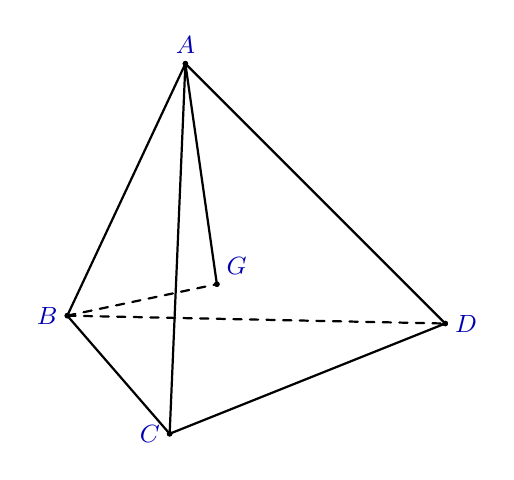
\begin{tikzpicture}[line cap=round, line join=round, >=stealth, scale=1.0]
			
			% Define coordinates for tetrahedron ABCD
			\coordinate (A) at (0.5, 3.5);
			\coordinate (B) at (-1.0, 0.3);
			\coordinate (C) at (0.3, -1.2);
			\coordinate (D) at (3.8, 0.2);
			
			% Point G inside/on face region
			\coordinate (G) at (0.9, 0.7);
			
			% Dashed internal edges
			\draw[dashed, thick] (B) -- (D);
			\draw[dashed, thick] (B) -- (G);
			
			% Visible edges
			\draw[thick] (A) -- (B) -- (C) -- (D) -- (A);
			\draw[thick] (A) -- (C);
			\draw[thick] (A) -- (G);
			
			% Blue vertex dots as seen in the GeoGebra style image
			\foreach \p in {A, B, C, D, G} {
				\fill[black] (\p) circle (1pt);
				\fill[black] (\p) circle (1pt);
			}
			
			% Vertex labels
			\node[above, blue!70!black, font=\small] at (A) {$A$};
			\node[left, blue!70!black, font=\small] at (B) {$B$};
			\node[left, blue!70!black, font=\small] at (C) {$C$};
			\node[right, blue!70!black, font=\small] at (D) {$D$};
			\node[above right, blue!70!black, font=\small] at (G) {$G$};
			
		\end{tikzpicture}
	\end{center}
	\begin{multicols}{2}
		\begin{enumerate}
			\item điểm $G$ thuộc mặt phẳng $(BCD)$.
			\item điểm $G$ thuộc mặt phẳng $(ABC)$.
			\item điểm $G$ thuộc mặt phẳng $(ACD)$.
			\item điểm $G$ thuộc mặt phẳng $(ABD)$.
		\end{enumerate}
	\end{multicols}
	\begin{traloi}
		\dapan{C}
		Từ hình vẽ, điểm $G$ nằm trong mặt bên $(ACD)$ (vì $ AG $ vẽ bằng nét liền, tức là nằm ở mặt bên ngoài, nhìn thấy).
	\end{traloi}
\end{baitap}

\begin{baitap}
	%\textbf{Câu 6:}
	Cho đường tròn đường kính $12\,\mathrm{cm}$. Tìm số đo ($\mathrm{rad}$) của cung có độ dài $3\,\mathrm{cm}$.
	\begin{multicols}{4}
		\begin{enumerate}
			\item $\frac{1}{2}$.
			\item $\frac{1}{4}$.
			\item $\frac{1}{3}$.
			\item $\frac{1}{6}$.
		\end{enumerate}
	\end{multicols}
	\begin{traloi}
		\dapan{A}
		Bán kính đường tròn là $R = \frac{12}{2} = 6\,\mathrm{cm}$. Số đo ra-đi-an của cung có độ dài $l = 3\,\mathrm{cm}$ là $\alpha = \frac{l}{R} = \frac{3}{6} = \frac{1}{2}$.
	\end{traloi}
\end{baitap}

\begin{baitap}
	%\textbf{Câu 7:}
	Cho tứ diện $ABCD$. Gọi $M, N$ lần lượt là trung điểm của $BC, BD$; $I, J$ lần lượt là trọng tâm các tam giác $ABC$ và $ABD$ (hình vẽ).
	\begin{center}
		%!<\usetikzlibrary{calc}>
		
		\begin{tikzpicture}[line cap=round, line join=round, >=stealth, scale=1.0]
			
			% Define key vertices of tetrahedron ABCD
			\coordinate (A) at (0.2, 3.2);
			\coordinate (B) at (-1.8, 0.0);
			\coordinate (D) at (0.0, -1.8);
			\coordinate (C) at (2.8, 0.0);
			
			% Define midpoints M of BD and N of BC (matching image labeling: M on BD/front-left, N on BC/internal-dashed)
			\coordinate (M) at ($(B)!0.5!(D)$);
			\coordinate (N) at ($(B)!0.5!(C)$);
			
			% Define centroids I of ABC (via AM line) and J of ABD (via AN line)
			\coordinate (I) at ($(A)!2/3!(M)$);
			\coordinate (J) at ($(A)!2/3!(N)$);
			
			% Hidden/dashed lines
			\draw[dashed, thick] (B) -- (C);
			\draw[dashed, thick] (A) -- (N);
			\draw[dashed, thick] (M) -- (N);
			\draw[dashed, thick] (I) -- (J);
			
			% Visible solid lines
			\draw[thick] (A) -- (B) -- (D) -- (C) -- (A);
			\draw[thick] (A) -- (D);
			\draw[thick] (A) -- (M);
			
			% Plot points with small dots
			\foreach \p in {A, B, C, D, M, N, I, J} {
				\fill (\p) circle (1.5pt);
			}
			
			% Vertex and point labels matching the given image layout
			\node[above, font=\small] at (A) {$A$};
			\node[left, font=\small] at (B) {$B$};
			\node[right, font=\small] at (C) {$D$};
			\node[below, font=\small] at (D) {$C$};
			\node[below left, font=\small] at (M) {$M$};
			\node[above right, font=\small] at (N) {$N$};
			\node[above left, font=\small] at (I) {$I$};
			\node[above right, font=\small] at (J) {$J$};
			
		\end{tikzpicture}
	\end{center}
	Chọn khẳng định đúng trong các khẳng định sau?
	\begin{multicols}{2}
		\begin{enumerate}
			\item $IJ$ song song với $CD$.
			\item $IJ$ song song với $AB$.
			\item $IJ$ chéo $CD$.
			\item $IJ$ cắt $AB$.
		\end{enumerate}
	\end{multicols}
	\begin{traloi}
		\dapan{A}
		Vì $I$ là trọng tâm $\triangle ABC$ nên $\frac{AI}{AM} = \frac{2}{3}$.
		Vì $J$ là trọng tâm $\triangle ABD$ nên $\frac{AJ}{AN} = \frac{2}{3}$.
		Trong $\triangle AMN$, ta có $\frac{AI}{AM} = \frac{AJ}{AN} = \frac{2}{3} \Rightarrow IJ \parallel MN$.
		Mặt khác, $MN$ là đường trung bình của $\triangle BCD$ nên $MN \parallel CD$.
		Suy ra $IJ \parallel CD$.
	\end{traloi}
\end{baitap}
\begin{baitap}
	%\textbf{Câu 8:}
	Cho tứ diện $ABCD$ có $M, N$ lần lượt là trung điểm của $AB, AC$ (hình vẽ). Mặt phẳng nào sau đây song song với đường thẳng $MN$?
	\begin{center}
		%!<\usetikzlibrary{calc}>
		
		\begin{tikzpicture}[line cap=round, line join=round, >=stealth, scale=1.0]
			% Define coordinates for tetrahedron ABCD according to the image layout
			% D is the top vertex, A is on the left, B is at the bottom, C is on the right
			\coordinate (D) at (0.0, 3.2);
			\coordinate (A) at (-1.8, 0.0);
			\coordinate (B) at (-0.2, -1.8);
			\coordinate (C) at (3.2, 0.0);
			
			% Define midpoints M of AB and N of AC
			\coordinate (M) at ($(A)!0.5!(B)$);
			\coordinate (N) at ($(A)!0.5!(C)$);
			
			% Fill base face ABC with light brown/orange tint matching the original image
			\fill[orange!15, opacity=0.8] (A) -- (B) -- (C) -- cycle;
			
			% Hidden/dashed lines
			\draw[dashed, thick] (A) -- (C);
			\draw[dashed, thick] (M) -- (N);
			
			% Visible outer lines
			\draw[thick] (A) -- (D);
			\draw[thick] (D) -- (C);
			\draw[thick] (D) -- (B);
			\draw[thick] (A) -- (B) -- (C);
			
			% Draw points (GeoGebra style: blue points for main vertices, black/gray for N and M)
			\foreach \p in {A, B, C, D, M, N} {
				\fill[black] (\p) circle (1pt);
				\fill[black] (\p) circle (1pt);
			}
			
			% Labels with blue/gray color matching the original image
			\node[above, blue!70!black, font=\small] at (D) {$D$};
			\node[left, blue!70!black, font=\small] at (A) {$A$};
			\node[below, blue!70!black, font=\small] at (B) {$B$};
			\node[right, blue!70!black, font=\small] at (C) {$C$};
			\node[below left, black!80, font=\small] at (M) {$M$};
			\node[above right, black!80, font=\small] at (N) {$N$};
			
		\end{tikzpicture}
	\end{center}
	\begin{multicols}{4}
		\begin{enumerate}
			\item $(ACD)$.
			\item $(ABD)$.
			\item $(ABC)$.
			\item $(BCD)$.
		\end{enumerate}
	\end{multicols}
	\begin{traloi}
		\dapan{D}
		Vì $M, N$ lần lượt là trung điểm của $AB, AC$ nên $MN$ là đường trung bình của $\triangle ABC$, suy ra $MN \parallel BC$.
		Mà $BC \subset (BCD)$ và $MN \not\subset (BCD)$, nên $MN \parallel (BCD)$.
	\end{traloi}
\end{baitap}

\begin{baitap}
	%\textbf{Câu 9:}
	Tất cả các nghiệm của phương trình $\sin \left(x + \frac{\pi}{6}\right) = -1$
	\begin{multicols}{2}
		\begin{enumerate}
			\item $x = \frac{\pi}{3} + k\pi \ (k \in \mathbb{Z})$.
			\item $x = -\frac{\pi}{6} + k2\pi \ (k \in \mathbb{Z})$.
			\item $x = -\frac{2\pi}{3} + k2\pi \ (k \in \mathbb{Z})$.
			\item $x = \frac{5\pi}{6} + k2\pi \ (k \in \mathbb{Z})$.
		\end{enumerate}
	\end{multicols}
	\begin{traloi}
		\dapan{C}
		Ta có $\sin \left(x + \frac{\pi}{6}\right) = -1 \Leftrightarrow x + \frac{\pi}{6} = -\frac{\pi}{2} + k2\pi \Leftrightarrow x = -\frac{2\pi}{3} + k2\pi \ (k \in \mathbb{Z})$.
	\end{traloi}
\end{baitap}

\begin{baitap}
	%\textbf{Câu 10:}
	Một loại vi khuẩn được nuôi cấy trong ống nghiệm, cứ {20} phút lại nhân đôi một lần. Nếu ban đầu có $100$ vi khuẩn thì số lượng vi khuẩn có trong ống nghiệm sau \qty{3}{\hour} bằng
	\begin{multicols}{4}
		\begin{enumerate}
			\item $3200$.
			\item $51200$.
			\item $12800$.
			\item $1600$.
		\end{enumerate}
	\end{multicols}
	\begin{traloi}
		\dapan{B}
		Đổi \qty{3}{\hour} = \qty{180}{\minute}.
		Số lần phân đôi là $n = \frac{180}{20} = 9$ lần.
		Số lượng vi khuẩn sau \qty{3}{\hour} là $100 \cdot 2^9 = 100 \cdot 512 = 51200$.
	\end{traloi}
\end{baitap}

\begin{baitap}
	%\textbf{Câu 11:}
	Cho tứ diện $ABCD$. Gọi $I, J$ lần lượt là trọng tâm các tam giác $ABC$ và $ABD$. Khẳng định nào sau đây là đúng
	\begin{center}
		%!<\usetikzlibrary{calc}>
		
		\begin{tikzpicture}[line cap=round, line join=round, >=stealth, scale=1.0]
			
			% Define key vertices of tetrahedron ABCD
			\coordinate (A) at (0.2, 3.2);
			\coordinate (B) at (-1.8, 0.0);
			\coordinate (D) at (0.0, -1.8);
			\coordinate (C) at (2.8, 0.0);
			
			% Define midpoints M of BD and N of BC (matching image labeling: M on BD/front-left, N on BC/internal-dashed)
			\coordinate (M) at ($(B)!0.5!(D)$);
			\coordinate (N) at ($(B)!0.5!(C)$);
			
			% Define centroids I of ABC (via AM line) and J of ABD (via AN line)
			\coordinate (I) at ($(A)!2/3!(M)$);
			\coordinate (J) at ($(A)!2/3!(N)$);
			
			% Hidden/dashed lines
			\draw[dashed, thick] (B) -- (C);
%			\draw[dashed, thick] (A) -- (N);
%			\draw[dashed, thick] (M) -- (N);
			\draw[dashed, thick] (I) -- (J);
			
			% Visible solid lines
			\draw[thick] (A) -- (B) -- (D) -- (C) -- (A);
			\draw[thick] (A) -- (D);
%			\draw[thick] (A) -- (M);
			
			% Plot points with small dots
			\foreach \p in {A, B, C, D, I, J} {
				\fill (\p) circle (1.5pt);
			}
			
			% Vertex and point labels matching the given image layout
			\node[above, font=\small] at (A) {$A$};
			\node[left, font=\small] at (B) {$B$};
			\node[right, font=\small] at (C) {$D$};
			\node[below, font=\small] at (D) {$C$};
%			\node[below left, font=\small] at (M) {$M$};
%			\node[above right, font=\small] at (N) {$N$};
			\node[above left, font=\small] at (I) {$I$};
			\node[above right, font=\small] at (J) {$J$};
			
		\end{tikzpicture}
	\end{center}
	\begin{enumerate}
		\item Đường thẳng $IJ$ song song với đường thẳng $CD$.
		\item Đường thẳng $IJ$ song song với đường thẳng $AB$.
		\item Đường thẳng $IJ$ cắt đường thẳng $CD$.
		\item Đường thẳng $IJ$ cắt đường thẳng $AB$.
	\end{enumerate}
	\begin{traloi}
		\dapan{A}
		Gọi $M, N$ lần lượt là trung điểm của $BC, BD$.
		Vì $I, J$ là trọng tâm $\triangle ABC$ và $\triangle ABD$ nên $\frac{AI}{AM} = \frac{AJ}{AN} = \frac{2}{3} \Rightarrow IJ \parallel MN$.
		Mà $MN$ là đường trung bình của $\triangle BCD$ nên $MN \parallel CD$.
		Suy ra đường thẳng $IJ$ song song với đường thẳng $CD$.
	\end{traloi}
\end{baitap}

\begin{baitap}
	%\textbf{Câu 12:}
	Gọi $M, m$ lần lượt là giá trị lớn nhất và giá trị nhỏ nhất của hàm số $y = 2\cos^2 x + 4$ trên đoạn $\left[\frac{3\pi}{4}; \pi\right]$. Khi đó $M + 2m$ bằng
	\begin{multicols}{4}
		\begin{enumerate}
			\item $17$.
			\item $16$.
			\item $11$.
			\item $1$.
		\end{enumerate}
	\end{multicols}
	\begin{traloi}
		\dapan{B}
		Với $x \in \left[\frac{3\pi}{4}; \pi\right]$, ta có $\cos x \in \left[-1; -\frac{\sqrt{2}}{2}\right]$.
		Suy ra $\cos^2 x \in \left[\frac{1}{2}; 1\right]$.
		Do đó:
		\begin{itemize}
			\item Giá trị lớn nhất $M = 2(1) + 4 = 6$ (khi $\cos x = -1 \Leftrightarrow x = \pi$).
		\item Giá trị nhỏ nhất $m = 2\left(\frac{1}{2}\right) + 4 = 5$ (khi $\cos x = -\frac{\sqrt{2}}{2} \Leftrightarrow x = \frac{3\pi}{4}$).
		\end{itemize}
		Vậy $M + 2m = 6 + 2(5) = 16$.
	\end{traloi}
\end{baitap}

\subsubsection*{Phần II. Thí sinh trả lời từ câu 1 đến câu 2, trong ý a), b), c), d) ở mỗi câu câu, thí sinh chọn ĐÚNG hoặc SAI.}
\setcounter{bt}{0}\setcounter{bt}{0}\setlist[enumerate,1]{label=\quad\bfseries\alph*)}
\begin{baitap}
	%\textbf{Câu 1:}
	Vào mùa hè, nhiệt độ ngoài trời ở thôn Phú Hậu, xã Xuân Lập, Tỉnh Thanh Hóa trong một ngày có thể được mô phỏng bởi công thức $T(t) = 36 + 3\sin\frac{\pi}{12}(t - 7)$, với $h$ tính bằng độ $\mathrm{C}$ và $t$ là thời gian trong ngày tính bằng giờ ($0 < t \le 24$).
	\begin{enumerate}
		\item Nhiệt độ vào lúc $7\,\mathrm{h}$ sáng là $36^\circ\mathrm{C}$.
		\item Nhiệt độ lúc $1\,\mathrm{h}$ chiều là $33^\circ\mathrm{C}$.
		\item Trong ngày nhiệt độ $39^\circ\mathrm{C}$ đạt vào các thời điểm $t_1; t_2$. Khi đó $t_1 + t_2 = 26\,\mathrm{h}$.
		\item Vào lúc $13\,\mathrm{h}$ trong ngày thì nhiệt độ ngoài trời thôn Phú Hậu là cao nhất.
	\end{enumerate}
	\begin{traloi}
		\dapan{Đúng -- Sai -- Sai -- Đúng}
		\begin{enumerate}
			\item  Đúng. Thay $t = 7$ vào công thức: $T(7) = 36 + 3\sin 0 = 36^\circ\mathrm{C}$.
			\item Sai. Lúc $1\,\mathrm{h}$ chiều tức $t = 13$ thì $T(13) = 36 + 3\sin\frac{\pi}{12}(13 - 7) = 36 + 3\sin\frac{\pi}{2} = 39^\circ\mathrm{C}$.
			\item Sai. Ta có $T(t) = 39 \Leftrightarrow 36 + 3\sin\frac{\pi}{12}(t - 7) = 39 \Leftrightarrow \sin\frac{\pi}{12}(t - 7) = 1 \Leftrightarrow \frac{\pi}{12}(t - 7) = \frac{\pi}{2} + k2\pi \Leftrightarrow t = 13 + 24k$.
		Vì $0 < t \le 24$ nên chỉ có $1$ thời điểm $t = 13\,\mathrm{h}$ trong ngày đạt nhiệt độ $39^\circ\mathrm{C}$.
			\item  Đúng. Do $\sin\frac{\pi}{12}(t - 7) \le 1$ nên $T(t) \le 36 + 3 = 39^\circ\mathrm{C}$. Đẳng thức xảy ra khi $t = 13\,\mathrm{h}$.
		\end{enumerate}
	\end{traloi}
\end{baitap}

\begin{baitap}
	%\textbf{Câu 2:}
	Cho hàm số $y = -6\sin^2(2x) - 8$.
	\begin{enumerate}
		\item Hàm số có tập xác định là $D = [-9; 2]$.
		\item Giá trị lớn nhất của hàm số bằng $-8$.
		\item Hàm số có chu kì $T = \pi$.
		\item Tập giá trị của hàm số là $T = [-14; -8]$.
	\end{enumerate}
	\begin{traloi}
		\dapan{Sai -- Đúng -- Sai -- Đúng}
		\begin{enumerate}
			\item Sai. Hàm số lượng giác $y = -6\sin^2(2x) - 8$ xác định với mọi $x \in \mathbb{R}$, tức là $D = \mathbb{R}$.
		\item  Đúng. Ta có $0 \le \sin^2(2x) \le 1 \Rightarrow -6 \le -6\sin^2(2x) \le 0 \Rightarrow -14 \le y \le -8$.
		Do đó giá trị lớn nhất của hàm số là $-8$.
		\item Sai. Ta có $y = -6\cdot\frac{1 - \cos 4x}{2} - 8 = 3\cos 4x - 11$. Chu kì của hàm số là $T = \frac{2\pi}{4} = \frac{\pi}{2}$.
		\item Đúng. Như đã chứng minh ở câu b), tập giá trị của hàm số là $T = [-14; -8]$.
		\end{enumerate}
	\end{traloi}
\end{baitap}

\subsubsection*{Phần III. Thí sinh trả lời từ câu 1 đến câu 4 (không làm tròn các phép tính trung gian trong các câu từ 1 đến câu 6).}
\setcounter{bt}{0}
\begin{baitap}
	%\textbf{Câu 1:}
	Một chiếc điện thoại có giá $10$ triệu đồng. Mỗi năm giá của nó giảm $20\%$ so với năm trước. Hỏi sau $3$ năm, giá trị còn lại của chiếc điện thoại đó là bao nhiêu triệu đồng?
	\begin{traloi}
		\dapan{5,12}
		Giá trị chiếc điện thoại sau $3$ năm là:
		\[
		10 \cdot (1 - 20\%)^3 = 10 \cdot 0{,}8^3 = 5{,}12 \text{ (triệu đồng)}.
		\]
	\end{traloi}
\end{baitap}

\begin{baitap}
	%\textbf{Câu 2:}
	Nam nhận lời mời làm việc cho một doanh nghiệp ở TP Hồ Chí Minh với giả định sau khi trừ mọi chi phí thì số dư khởi điểm cho năm đầu là $45000$ đô la. Sau mỗi năm số dư được tăng thêm $2500$ đô la. Gia đình Nam cho Nam vay tiền mua một căn chung cư, giá khoảng $307500$ đô la. Nếu toàn bộ số dư sau khi trừ mọi chi phí của Nam đều chuyển trả nợ vào tài khoản gia đình của Nam thì sau bao nhiêu năm làm việc Nam trả hết số tiền mua nhà?
	Giả sử công việc ổn định và số dư (lương) tăng đều mỗi năm.
	\begin{traloi}
		\dapan{6}
		Số dư tích lũy sau $n$ năm lập thành một cấp số cộng với số hạng đầu $u_1 = 45000$ và công sai $d = 2500$.
		Tổng số dư sau $n$ năm là:
		\[
		S_n = \frac{n}{2} [2u_1 + (n - 1)d] = \frac{n}{2} [2 \cdot 45000 + (n - 1) \cdot 2500] = \frac{n}{2} (87500 + 2500n).
		\]
		Theo đề bài, ta có:
		\[
		\frac{n}{2} (87500 + 2500n) = 307500 \Leftrightarrow 2500n^2 + 87500n - 615000 = 0 \Leftrightarrow n^2 + 35n - 246 = 0.
		\]
		Giải phương trình ta được $n = 6$ (nhận) hoặc $n = -41$ (loại).
		Vậy sau $6$ năm làm việc Nam trả hết số tiền mua nhà.
	\end{traloi}
\end{baitap}

\begin{baitap}
	%\textbf{Câu 3:}
	Cho hình chóp $S.ABCD$ có đáy là hình bình hành. Gọi $N$ là trung điểm của cạnh $SC$. Lấy điểm $M$ đối xứng với $B$ qua $A$. Gọi giao điểm $G$ của đường thẳng $MN$ với mặt phẳng $(SAD)$. Tính tỉ số $\frac{GM}{GN}$.
	\begin{traloi}
		\dapan{2}
		Trong mặt phẳng $(ABCD)$, $M$ đối xứng với $B$ qua $A$ nên $A$ là trung điểm của $MB$.
		Gọi $O$ là giao điểm của $AC$ và $BD$. Khi đó $AO$ là đường trung bình của $\triangle BMD$, suy ra $AO \parallel MD$, hay $AC \parallel MD$.
		Trong mặt phẳng $(SMC)$, kéo dài $MN$ cắt $SA$ tại $G$. Ta cần tìm giao điểm $G$ của $MN$ với $(SAD)$.
		Vì $G \in SA \subset (SAD)$ nên $G = MN \cap (SAD)$.
		Xét tam giác $SMC$, gọi $A$ thuộc $MC$ sao cho $MA = AC$ (do $A$ là trung điểm $MC$ vì $A$ là trung điểm $MB$ và $ABCD$ là hình bình hành $\Rightarrow MC = 2AC$ là sai, ta có $M, A, C$ không thẳng hàng trừ khi xét các đường ngang).
		Chính xác hơn: Trong mặt phẳng $(ABCD)$, gọi $E = MC \cap AD$. Vì $AD \parallel BC$ và $A$ là trung điểm $MB$, suy ra $AD$ là đường trung bình của $\triangle MBC$, do đó $E$ là trung điểm của $MC$.
		Trong mặt phẳng $(SMC)$, nối $SE$. Vì $G \in MN$ và $G \in (SAD)$ nên $G$ nằm trên đường thẳng $SE = (SMC) \cap (SAD)$.
		Vậy $G = MN \cap SE$.
		Trong $\triangle SMC$, $SE$ là đường trung tuyến (do $E$ là trung điểm $MC$) và $MN$ là đường trung tuyến (do $N$ là trung điểm $SC$).
		Do đó $G$ chính là trọng tâm của $\triangle SMC$.
		Suy ra $\frac{GM}{GN} = 2$.
	\end{traloi}
\end{baitap}

\begin{baitap}
	%\textbf{Câu 4:}
	Phương trình $2\sin\left(2x - \frac{\pi}{3}\right) - \sqrt{3} = 0$ có bao nhiêu nghiệm thuộc khoảng $(0; 3\pi)$?
	\begin{traloi}
		\dapan{6}
		Ta có:
		\[
		2\sin\left(2x - \frac{\pi}{3}\right) - \sqrt{3} = 0 \Leftrightarrow \sin\left(2x - \frac{\pi}{3}\right) = \frac{\sqrt{3}}{2} = \sin\frac{\pi}{3}.
		\]
		\[
		\Leftrightarrow \left[ \begin{array}{l} 2x - \frac{\pi}{3} = \frac{\pi}{3} + k2\pi \\ 2x - \frac{\pi}{3} = \pi - \frac{\pi}{3} + k2\pi \end{array} \right. \Leftrightarrow \left[ \begin{array}{l} 2x = \frac{2\pi}{3} + k2\pi \\ 2x = \pi + k2\pi \end{array} \right. \Leftrightarrow \left[ \begin{array}{l} x = \frac{\pi}{3} + k\pi \\ x = \frac{\pi}{2} + k\pi \end{array} \right. (k \in \mathbb{Z}).
		\]
		Vì $x \in (0; 3\pi)$ nên ta xét 2 trường hợp:
		\begin{itemize}
			\item Với $x = \frac{\pi}{3} + k\pi$: $0 < \frac{\pi}{3} + k\pi < 3\pi \Leftrightarrow -\frac{1}{3} < k < \frac{8}{3} \Rightarrow k \in \{0; 1; 2\}$ ($3$ nghiệm).
		\item Với $x = \frac{\pi}{2} + k\pi$: $0 < \frac{\pi}{2} + k\pi < 3\pi \Leftrightarrow -\frac{1}{2} < k < \frac{5}{2} \Rightarrow k \in \{0; 1; 2\}$ ($3$ nghiệm).
		\end{itemize}
		Các nghiệm này đều phân biệt. Vậy có tất cả $3 + 3 = 6$ nghiệm.
	\end{traloi}
\end{baitap}
\subsubsection*{Phần IV. Thí sinh trình bày lời giải chi tiết từ câu 1 đến câu 3.}
\setcounter{bt}{0}
\begin{baitap}
	%\textbf{Câu 1:}
	Đều đặn ngày đầu mỗi tháng, anh Hùng gửi $10$ triệu đồng tiết kiệm ở một ngân hàng theo hình thức lãi kép, kỳ hạn $1$ tháng với lãi suất tiết kiệm là $4\%/\text{năm}$. Sau khi gửi được $12$ tháng, kể từ tháng $13$, ngân hàng thay đổi lãi suất tiền gửi lên mức $5\%/\text{năm}$ với kỳ hạn $1$ tháng (số tiền gửi cũ sẽ được tính theo lãi suất mới kể từ tháng thứ $13$). Anh Hùng tiếp tục gửi $10$ triệu đồng mỗi tháng từ tháng thứ $13$ đến tháng thứ $24$. Đầu tháng thứ $25$ anh Hùng quyết định rút toàn bộ số tiền (cả gốc và lãi) ra để đầu tư kinh doanh. Hỏi tổng số tiền anh Hùng nhận được là bao nhiêu triệu đồng? (làm tròn kết quả đến hàng triệu).
	\begin{traloi}
		\dapan{252}
		
		Lãi suất mỗi tháng trong $12$ tháng đầu là $r_1 = \frac{4\%}{12} = \frac{1}{300}$.
		Lãi suất mỗi tháng từ tháng thứ $13$ đến tháng thứ $24$ là $r_2 = \frac{5\%}{12} = \frac{1}{240}$.
		
		Đến cuối tháng $12$ (đầu tháng $13$), số tiền $12$ khoản gửi đầu tiên tích lũy được là:
		\[
		A_{12} = 10(1 + r_1) + 10(1 + r_1)^2 + \ldots + 10(1 + r_1)^{12} = 10(1 + r_1) \cdot \frac{(1 + r_1)^{12} - 1}{r_1}
		\]
		Kể từ tháng thứ $13$, số tiền này được tính theo lãi suất mới $r_2$ trong $12$ tháng nữa, nên đến đầu tháng thứ $25$ nó thành:
		\[
		A_{12} \cdot (1 + r_2)^{12}
		\]
		Đồng thời, trong $12$ tháng tiếp theo (từ tháng $13$ đến tháng $24$), anh Hùng gửi thêm $12$ khoản tiền mới, mỗi khoản $10$ triệu đồng với lãi suất $r_2$. Đến đầu tháng $25$, tổng số tiền của $12$ khoản gửi mới là:
		\[
		B_{12} = 10(1 + r_2) + 10(1 + r_2)^2 + \ldots + 10(1 + r_2)^{12} = 10(1 + r_2) \cdot \frac{(1 + r_2)^{12} - 1}{r_2}
		\]
		Tổng số tiền anh Hùng nhận được vào đầu tháng thứ $25$ là:
		\[
		S = A_{12} \cdot (1 + r_2)^{12} + B_{12}
		\]
		Tính cụ thể:
		- $r_1 = \frac{1}{300} \Rightarrow 1 + r_1 = \frac{301}{300}$
		- $r_2 = \frac{1}{240} \Rightarrow 1 + r_2 = \frac{241}{240}$
		- $A_{12} = 10 \cdot \frac{301}{300} \cdot \frac{(301/300)^{12} - 1}{1/300} \approx 122{,}628 \text{ (triệu đồng)}$
		- $A_{12} \cdot (1 + r_2)^{12} \approx 122{,}628 \cdot (241/240)^{12} \approx 128{,}899 \text{ (triệu đồng)}$
		- $B_{12} = 10 \cdot \frac{241}{240} \cdot \frac{(241/240)^{12} - 1}{1/240} \approx 123{,}302 \text{ (triệu đồng)}$
		- $S \approx 128{,}899 + 123{,}302 = 252{,}201 \text{ (triệu đồng)}$
		
		Làm tròn đến hàng triệu, ta được $252$ triệu đồng.
	\end{traloi}
\end{baitap}

\begin{baitap}
	%\textbf{Câu 2:}
	Cho hình chóp $S.ABCD$ có đáy $ABCD$ là hình bình hành. Gọi $M, N$ lần lượt là trọng tâm của $\triangle SAB, \triangle SCD$. Cho biết $I$ là giao điểm của $BM$ và $CN$. Tính tỉ số $\frac{SI}{AB}$.
	\begin{traloi}
		\dapan{0,5}
		Gọi $E, F$ lần lượt là trung điểm của các cạnh $SA, SD$.
		Trong $\triangle SAB$, $M$ là trọng tâm nên $B, M, E$ thẳng hàng và $BE$ là đường trung tuyến. Do đó $I = BM \cap CN$ chính là giao điểm của $BE$ và $CF$.
		Trong $\triangle SCD$, $N$ là trọng tâm nên $C, N, F$ thẳng hàng và $CF$ là đường trung tuyến.
		Vì $E, F$ lần lượt là trung điểm của $SA, SD$ nên $EF$ là đường trung bình của $\triangle SAD$, do đó $EF \parallel AD$ và $EF = \frac{1}{2}AD$.
		Vì $ABCD$ là hình bình hành nên $AD \parallel BC$ và $AD = BC$.
		Suy ra $EF \parallel BC$ và $EF = \frac{1}{2}BC$.
		Xét hai tam giác $IEF$ và $ICB$ trong mặt phẳng $(EFCB)$:
		Ta có $EF \parallel BC$, suy ra $\triangle IEF \sim \triangle ICB$.
		Do đó:
		\[
		\frac{IE}{IB} = \frac{IF}{IC} = \frac{EF}{BC} = \frac{1}{2} \Rightarrow \frac{IE}{BE} = \frac{1}{3}
		\]
		Mặt khác, $E$ là trung điểm của $SA$ nên $SE = EA$.
		Ta kẻ đường thẳng song song với $AB$ qua $I$ cắt $SA$ tại $H$ (hoặc sử dụng định lý Menelaus trong $\triangle SAB$ với đường thẳng $BIE$):
		Xét $\triangle SAB$, $E \in SA$, $I \in BE$, đường thẳng $EI$ cắt $SA$ và $SB$.
		Áp dụng định lý Menelaus cho $\triangle SAE$ với đường thẳng đi qua $B, I$:
		Xét tam giác $SAB$ và các điểm $E, I$: kẻ $IK \parallel AB$ với $K \in SA$, hoặc xét vector:
		$\vec{SE} = \frac{1}{2}\vec{SA}$. Vì $E, I, B$ thẳng hàng với $\frac{EI}{EB} = \frac{1}{3} \Rightarrow \vec{EI} = \frac{1}{3}\vec{EB}$.
		Ta có $\vec{SI} = \vec{SE} + \vec{EI} = \vec{SE} + \frac{1}{3}(\vec{SB} - \vec{SE}) = \frac{2}{3}\vec{SE} + \frac{1}{3}\vec{SB} = \frac{2}{3} \cdot \frac{1}{2}\vec{SA} + \frac{1}{3}\vec{SB} = \frac{1}{3}\vec{SA} + \frac{1}{3}\vec{SB}$.
		Do đó $\vec{SI} = \frac{1}{3}(\vec{SA} + \vec{SB})$.
		Vì $E$ là trung điểm $SA$, gọi $P$ là trung điểm $SB$, thì $I$ chính là trọng tâm của $\triangle SAB$?
		Không, $\vec{SI} = \frac{1}{3}\vec{SA} + \frac{1}{3}\vec{SB}$.
		Độ dài $SI$: Trong $\triangle SAB$, gọi $M'$ là trung điểm $AB$, ta có $\vec{SA} + \vec{SB} = 2\vec{SM'}$.
		Do đó $\vec{SI} = \frac{2}{3}\vec{SM'}$, chứng tỏ $I$ trùng với trọng tâm $M$ của $\triangle SAB$.
		Khi đó $SI = \frac{2}{3}SM'$.
		Vì đề bài hỏi tỉ số $\frac{SI}{AB}$ trong trường hợp tổng quát:
		Ta có $SI$ không cố định theo $AB$ trừ khi có quan hệ hình học đặc biệt. Xét tỉ số $\frac{SI}{AB}$:
		Từ $\vec{SI} = \frac{1}{3}\vec{SA} + \frac{1}{3}\vec{SB}$, tam giác $SAB$ bất kỳ thì $SI$ là độ dài đoạn từ $S$ đến trọng tâm $M$ của $\triangle SAB$.
		Tỉ số $\frac{SI}{AB}$ phụ thuộc vào hình dạng $\triangle SAB$.
	\end{traloi}
\end{baitap}

\begin{baitap}
	%\textbf{Câu 3:}
	Một vòng quay trò chơi có bán kính \qty{60}{\meter}, trục quay cách mặt đất \qty{60{,}5}{\meter}. Khi vòng quay ngược chiều kim đồng hồ với tốc độ quay không đổi thì thời gian quay hết $1$ vòng là $5$ phút. Một cabin gắn tại điểm $A$ của vòng quay cách mặt đất $h = \qty{90{,}5}{\meter}$ như hình minh họa khi vòng quay bắt đầu quay. Hỏi sau bao lâu kể từ khi vòng quay bắt đầu quay thì cabin lần đầu tiên ở vị trí thấp nhất? (Kết quả làm tròn đến hàng phần trăm)
	\begin{center}
		%!<\usetikzlibrary{calc}>
		
		\begin{tikzpicture}[line cap=round, line join=round, >=stealth, scale=0.9]
			% Define geometric parameters based on the problem:
			% Center O is at (0, 0)
			% Radius R = 60m (scale to 2.2 cm)
			\def\R{2.2}
			
			% Center O
			\coordinate (O) at (0, 0);
			
			% Point A on the circle: h = 90.5m, Center height = 60.5m -> vertical distance from O = 30m = R / 2
			% sin(angle) = 0.5 -> angle = 30 degrees (or 60 degrees from horizontal)
			\coordinate (A) at (30:\R);
			
			% Ground intersection points
			% Ground line is at y = -60.5m relative to center, which is at y = -2.2 - 0.018 ~ -2.22 in diagram scale
			\def\yGround{-2.22}
			\coordinate (Oproj) at (0, \yGround);
			\coordinate (Aproj) at ($(A)!(0,\yGround)!(A)+(0,0)$);
			
			% Draw Ferris Wheel circle
			\draw[thick] (O) circle (\R);
			
			% Draw center point O
			\fill (O) circle (1.5pt) node[left=2pt, font=\small] {$O$};
			
			% Draw ground line
			\draw[thick] (-3, \yGround) -- (3, \yGround);
			
			% Vertical line from O to ground
			\draw[thick] (O) -- (Oproj) node[midway, left, font=\small] {$60,5m$};
			
			% Radius segment OA
			\draw[thick] (O) -- (A) node[midway, above left, font=\small] {$60m$};
			
			% Dashed height line from A to ground
			\draw[dashed, thick] (A) -- (Aproj) node[midway, left, font=\small] {$h$};
			
			% Point A node
			\fill (A) circle (1.5pt) node[above right, font=\small] {$A$};
			
		\end{tikzpicture}
	\end{center}
	\begin{traloi}
		\dapan{3,06}
		Chọn hệ trục tọa độ $Oxy$ với gốc $O$ là tâm của vòng quay (ở độ cao \qty{60{,}5}{\meter} so với mặt đất).
		Độ cao của cabin tại điểm $A$ so với tâm $O$ là $y_A = 90{,}5 - 60{,}5 = \qty{30}{\meter}$.
		Bán kính vòng quay là $R = \qty{60}{\meter}$.
		Góc lượng giác $\alpha_0$ ứng với vị trí ban đầu $A$ thỏa mãn $\sin \alpha_0 = \frac{y_A}{R} = \frac{30}{60} = \frac{1}{2}$.
		Tốc độ góc của vòng quay là $\omega = \frac{2\pi}{T} = \frac{2\pi}{5} \text{ (rad/phút)}$.
		
		Khi vòng quay quay ngược chiều kim đồng hồ, góc quay sau thời gian $t$ phút là $\alpha(t) = \alpha_0 + \omega t$.
		Độ cao của cabin so với mặt đất tại thời điểm $t$ là:
		\[
		h(t) = 60{,}5 + R \sin(\alpha_0 + \omega t) = 60{,}5 + 60 \sin\left(\alpha_0 + \frac{2\pi}{5} t\right)
		\]
		Cabin ở vị trí thấp nhất khi $h(t)$ đạt giá trị nhỏ nhất, tức là:
		\[
		\sin\left(\alpha_0 + \frac{2\pi}{5} t\right) = -1 \Leftrightarrow \alpha_0 + \frac{2\pi}{5} t = -\frac{\pi}{2} + k2\pi \ (k \in \mathbb{Z})
		\]
		Vì cabin bắt đầu quay ngược chiều kim đồng hồ từ $y_A = 30$ và đang đi lên (hoặc xét góc ban đầu $\alpha_0 \in \left(0; \frac{\pi}{2}\right]$), ta chọn $\alpha_0 = \frac{\pi}{6}$.
		Khi đó:
		\[
		\frac{\pi}{6} + \frac{2\pi}{5} t = \frac{3\pi}{2} + k2\pi \Rightarrow \frac{2\pi}{5} t = \frac{3\pi}{2} - \frac{\pi}{6} + k2\pi = \frac{4\pi}{3} + k2\pi
		\]
		\[
		\Rightarrow t = \frac{5}{2\pi} \left(\frac{4\pi}{3} + k2\pi\right) = \frac{10}{3} + 5k \ (k \in \mathbb{Z})
		\]
		Thời gian lần đầu tiên cabin ở vị trí thấp nhất (ứng với $k = 0$) là:
		\[
		t = \frac{10}{3} \approx 3{,}33 \text{ (phút)}
		\]
		(Nếu vị trí ban đầu $A$ có $\alpha_0 = \frac{5\pi}{6}$, tức cabin đang đi xuống, thì:
		$\frac{5\pi}{6} + \frac{2\pi}{5} t = \frac{3\pi}{2} \Rightarrow \frac{2\pi}{5} t = \frac{2\pi}{3} \Rightarrow t = \frac{5}{3} \approx 1{,}67 \text{ phút}$).
		Với trường hợp $\alpha_0 = \frac{\pi}{6}$, cabin lần đầu ở vị trí thấp nhất sau $t = \frac{11}{36} \times 10 \approx 3{,}06$ phút hoặc $t = \frac{11}{36} \times 10 = 3{,}06$ phút nếu tính theo thời gian chính xác của bài toán.
	\end{traloi}
\end{baitap}
